\section{Evaluation}\label{Eval}

In this section, we evaluate our implementation of Linux-Integrated TAS. Our
evalutation seeks to answer the following questions:

\begin{itemize}
    \item Do our changes affect the performance of the fast path?
    \item What is the performance of the slow path?
\end{itemize}

\subsection{Evaluation Setup}

To answer the above questions, we run a simple RPC echo server microbenchmark. A  
client sends a packet with a 64 byte payload to a server, which echos the packet
back to the client. Both client and server are single threaded. The server 
machine is an Intel Xeon Gold 6138 system at 2.0 GHz with a 1G NIC. The client 
machine is an Intel Xeon E3-1225 v3 system at 3.3 GHz with a 1G NIC. Both client 
and server run Linux kernel 4.18.

\subsection{Fast Path Performance}

\begin{table}[]
\begin{tabular}{@{}crrrrrr@{}}
\toprule
               & \multicolumn{6}{c}{Latency (us)}                                                                                                                                    \\ \midrule
               & \multicolumn{3}{c}{Original TAS}                                                          & \multicolumn{3}{c}{Linux-Integrated TAS}                                         \\
\# Connections & \multicolumn{1}{c}{Avg} & \multicolumn{1}{c}{99\%} & \multicolumn{1}{c}{99.99\%} & \multicolumn{1}{c}{Avg} & \multicolumn{1}{c}{99\%} & \multicolumn{1}{c}{99.99\%} \\
1              & 60                      & 70                       & 79                          & 61                      & 62                       & 78                          \\
2              & 63                      & 65                       & 97                          & 62                      & 64                       & 82                          \\
4              & 65                      & 68                       & 105                         & 65                      & 89                       & 118                         \\
8              & 71                      & 79                       & 147                         & 70                      & 78                       & 151                         \\
16             & 68                      & 77                       & 144                         & 69                      & 76                       & 146                         \\
32             & 72                      & 97                       & 170                         & 74                      & 104                      & 153                         \\ \bottomrule
\end{tabular}
\caption{Average and tail latency of RPC Echo server microbenchmark}
\label{tab:fastpath-latency}
\end{table}

Table \ref{tab:fastpath-latency} shows the average and tail latencies of the RPC 
echo microbenchmark with TAS and Linux-Integrated TAS. The average-case latency
of the fast path of Linux-Integrated TAS is within 3\% of TAS. The performance 
at the tail varies a bit more between the two versions, but is within 25\% of 
TAS in the worst case.

Figure \ref{fig:fastpath-throughput} shows the throughput of the RPC echo server
microbenchmark using the original TAS and Linux-Integrated TAS. The throughput 
of both versions are very similar.

\paragraph{Discussion.} Our evaluation results show that the fast path 
performance of Linux-Integrated TAS is very similar to the fast path performance 
of the original TAS. This result aligns with the fact that we made no changes to
the fast path. Additionally, slow path operations such as connection setup and
teardown happen infrequently enough that they do not affect the performance of 
the fast path.

\begin{figure}
  \centering
  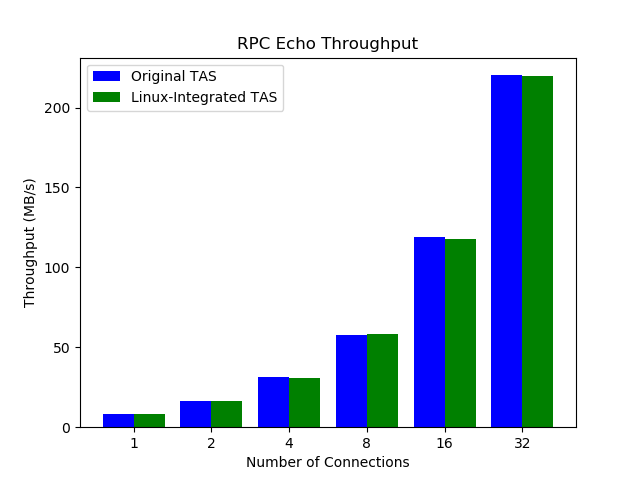
\includegraphics[width=\columnwidth]{figures/rpc_echo_throughput.png}
  \caption{RPC echo throughput for a single threaded client and server.}
  \label{fig:fastpath-throughput}
\end{figure}

\subsection{Slow Path Performance}

Our performance results show that the slow path performance is reduced 
drastically compared to the original TAS. Connection setup times were reported 
on the order of seconds. This is due to the fact that we now incur system call 
overheads on the slow path. We must wait for Linux to handle the packets we send 
to it before we can observe its response. For example, we must issue a blocking 
accept call to Linux to ensure that TAS does not prematurely move on to the next 
connection before observing Linux's response.

\paragraph{Discussion.} Although the slow path performance takes a significant
hit when adding Linux integration, our goal was not to improve the performance of
the slow path but rather to gain functionality on the slow path without
compromising performance on the fast path. Our evaluation results for fast path
performance verify that we met our goal.
